%% Progetto di linguaggi di programmazione - Gianluca Grilletti e Giovanni Barbarino
%% Semantica Fully Abstract per PCF


\documentclass{beamer}

\usepackage[utf8]{inputenc}
\usepackage{default}
\usepackage{amssymb}
\usepackage{stmaryrd}
\usepackage{graphicx}
\usepackage{caption}
\usepackage{subcaption}
\usepackage{tikz}
\usetikzlibrary{arrows,automata}
\usepackage[usenames,dvipsnames]{color}

\newcommand{\eqobs}{\stackrel{\text{obs}}{=}}
\newcommand{\limp}{\mathbin{{-}\mkern-3.5mu{\circ}}}
\newcommand{\tnode}[4]{\node (#1_u) at (#2,#3+0.1) [minimum size=2pt, opacity=0] 		       {#4};
		       \node (#1_d) at (#2,#3-0.1) [minimum size=2pt, opacity=0] {#4};
		       \node (#1) at (#2,#3) [minimum size=2pt] {#4};}
\newcommand{\tavolo}[5]{\draw [fill=#1, opacity=.5] (#2,#3) rectangle (#4,#5);} 


% immagini
\graphicspath{{immagini/}}




\usetheme{Darmstadt}

\title{Un modello fully abstract del PCF}
% \subtitle{Vuoi fare un gioco con me?}
\author{Grilletti Gianluca \and Barbarino Giovanni}
\institute[Unipi]{Università di Pisa}


\begin{document}

\small


\section{Il linguaggio PCF}
\subsection{La sintassi}

%titolo
\begin{frame}
	%\frametitle{Il linguaggio PCF}
	\maketitle
	
\end{frame}



% tavolo e carte
\begin{frame}
	
	Come rappresentiamo i giochi (il tavolo insomma)
	
	\begin{tikzpicture}
	 \node (inv) at (0,0) [minimum size=2pt] {};
	 \node (inv2) at (6,-6) [minimum size=2pt, scale=1.5] {};
	 
	 \draw [fill=blue, opacity=.5] (7,-5) rectangle (3,-1);
	 \node (A) at (5,-3) [minimum size=2pt, scale=4] {A};
	 \node (P) at (3.5,-4.5) [minimum size=2pt, scale=2.5] {P};
	 \node (O) at (3.5,-1.5) [minimum size=2pt, scale=2.5] {O};
	 
	 
	 
	 \only<2-> {\node (st_1) at (6,-0.5) [minimum size=2pt, scale=1.5] {$*_1$};}
	 \only<3-> {\node (st_2) at (6,-5.5) [minimum size=2pt, scale=1.5] {$*_2$};}
	 \only<4->{\node (ri_1) at (4.5,-0.5) [minimum size=2pt, scale=1.5] {$n_2$};}
	 \only<5->{\node (ri_2) at (4.5,-5.5) [minimum size=2pt, scale=1.5] {$n_1$};}
	 
	  \only<3->{\draw[->] [out=280,in=80] (st_1) to (st_2);}
	  \only<4->{\draw[->] [out=110,in=300] (st_2) to (ri_1);}
	  \only<5->{\draw[->] [out=280,in=80] (ri_1) to (ri_2);}
	\end{tikzpicture}

	
	
	
\end{frame}


% prova di implicazione
\begin{frame}
	\[
	A \implies B \quad \equiv \quad !A \limp B
	\]
	\begin{tikzpicture}
	 \node (inv) at (0,0) [minimum size=2pt] {};
	 \node (inv2) at (11,-4) [minimum size=2pt] {};
	 \foreach \x in {0,3,6} { 
	  \draw [fill=SkyBlue] (\x+2,-3) rectangle (\x,-1);
	  \node (A\x) at (\x+1,-2) [minimum size=2pt, scale=2] {A};
	  \node (P\x) at (\x+0.3,-1.3) [minimum size=2pt, scale=1.5] {P};
 	  \node (O\x) at (\x+0.3,-2.7) [minimum size=2pt, scale=1.5] {O};
	  }
	 \draw [fill=red, opacity=.5] (11,-3) rectangle (9,-1);
	 \node (B) at (10,-2) [minimum size=2pt, scale=2] {B};
	 \node (P) at (9.3,-2.7) [minimum size=2pt, scale=1.5] {P};
 	 \node (O) at (9.3,-1.3) [minimum size=2pt, scale=1.5] {O};
	 
	 \only<2->{\node (st_1) at (10,-0.5) [minimum size=2pt, scale=1.5] {$*_1$};}
 	 \only<3->{\node (st_2) at (7,-0.5) [minimum size=2pt, scale=1.5] {$*_2$};}
	 \only<4->{\node (ri_2) at (7,-3.5) [minimum size=2pt, scale=1.5] {$n_2$};}
 	 \only<5->{\node (st_3) at (4,-0.5) [minimum size=2pt, scale=1.5] {$*_3$};}
	 \only<6->{\node (ri_3) at (4,-3.5) [minimum size=2pt, scale=1.5] {$n_3$};}
 	 \only<7->{\node (ri_1) at (10,-3.5) [minimum size=2pt, scale=1.5] {$n_1$};}
 	 
	  \only<3->{\draw[->] [out=250,in=280] (st_1) to (st_2);}
	  \only<4->{\draw[->] [out=250,in=30] (st_2) to (ri_2);}
	  \only<5->{\draw[->] [out=80,in=280] (ri_2) to (st_3);}
	  \only<6->{\draw[->] [out=250,in=110] (st_3) to (ri_3);}
	  \only<7->{\draw[->] [out=30,in=150] (ri_3) to (ri_1);}
	  \end{tikzpicture}

	
	
	
\end{frame}




\end{document}
